\documentclass[aspectratio=169,11pt,xcolor=dvipsnames]{beamer}
\usepackage{graphicx} % For including graphics.
\usepackage{hyperref} % For links.
\usepackage{multimedia}
\usepackage{transparent}
\usepackage{tikz}
\usepackage{minted}

\title{Volumetric Clouds with Clojure and LWJGL}
\subtitle{Clojure Jam 2026}
\author{Jan Wedekind}
\date{Saturday, April 18th 2026}

\hypersetup{pdftitle          = {Volumetric Clouds with Clojure and LWJGL},
            pdfsubject        = {Rendering Volumetric Clouds using Clojure, LWJGL, Fastmath, and dtype-next},
            pdfauthor         = {Jan Wedekind},
            pdfkeywords       = {Clojure, LWJGL, Fastmath, dtype-next, volumetric clouds, rendering, graphics},
            pdfcreator        = {LaTeX with Beamer class},
            pdfproducer       = {TeX Live 2024 on Debian},
            bookmarksopen     = false,
            bookmarksnumbered = true,
            colorlinks        = true,
            filecolor         = cyan,
            citecolor         = green,
            linkcolor         = blue,
            urlcolor          = blue}

\pdfcompresslevel=9

\definecolor{slidecolor}{rgb}{0.65,0.71,0.72}
\definecolor{bluish}{rgb}{0.678,0.678,0.878}
\definecolor{lightred}{rgb}{1.0, 0.9, 0.9}


\usebackgroundtemplate{
  {\transparent{0.6}
\includegraphics[width=\paperwidth,height=\paperheight]{slide}}
  \begin{tikzpicture}[remember picture,overlay]
    \node[anchor=south west,yshift=-0.05cm,xshift=0.0cm] at (current page.south west) {
      \begin{tiny}
        \hypersetup{urlcolor=bluish}
        \url{https://www.wedesoft.de/downloads/clojure-clouds.pdf}
        \hypersetup{urlcolor=blue}
      \end{tiny}};
    \node[anchor=south, yshift=-0.05cm, xshift=0.0cm] at (current page.south) {
      \begin{tiny}
        \textcolor{bluish}{\insertframenumber/\inserttotalframenumber}
      \end{tiny}};
  \end{tikzpicture}
}

\setbeamersize{text margin left=0.5cm,
               text margin right=0.5cm}
\addtobeamertemplate{frametitle}{}{\vspace{-0.3cm}}

\usecolortheme{seahorse}

\setbeamercolor{titlelike}{fg=black,bg=slidecolor!60}
\setbeamercolor{frametitle}{fg=black,bg=slidecolor!100}

% pygmentize -L styles
\usemintedstyle{default}
\setminted{highlightcolor=lightred}

\begin{document}

\begin{frame}
  \pdfbookmark[1]{Title}{title}
  \begin{center}
  \titlepage{}
  \end{center}
\end{frame}

\begin{frame}[fragile]
  \frametitle{Noise Volume Parameters}
  \begin{minted}[]{clj}
(defn make-noise-params
  [size divisions dimensions]
  {:size size
   :divisions divisions
   :cellsize (/ size divisions)
   :dimensions dimensions})

(make-noise-params 256 8 2)
; {:size 256, :divisions 8, :cellsize 32, :dimensions 2}
  \end{minted}
\end{frame}

\begin{frame}[fragile]
  \frametitle{Generic Vector Constructor}
  \begin{minted}[]{clj}
(defn vec-n
  ([x y] (vec2 x y))
  ([x y z] (vec3 x y z)))

(vec-n 2 3)
; #vec2 [2.0, 3.0]
(vec-n 2 3 1)
; #vec3 [2.0, 3.0, 1.0]
  \end{minted}
\end{frame}

\begin{frame}
  \frametitle{Worley Noise}
  \begin{center}
    Worley noise / Voronoi noise
    \begin{itemize}
      \item Divide space into cell
      \item Place random point in each cell
      \item distance to closest point is Worley noise function
    \end{itemize}
  \end{center}
\end{frame}

\begin{frame}[fragile]
  \frametitle{Random Point in a Cell: Tests}
  \begin{minted}[]{clj}
(facts "Place random point in a cell"
   (with-redefs [rand (fn [s] (* 0.5 s))]
     (random-point-in-cell {:cellsize 1} 0 0) => (vec2 0.5 0.5)
     (random-point-in-cell {:cellsize 2} 0 0) => (vec2 1.0 1.0)
     (random-point-in-cell {:cellsize 2} 0 3) => (vec2 7.0 1.0)
     (random-point-in-cell {:cellsize 2} 2 0) => (vec2 1.0 5.0)
     (random-point-in-cell {:cellsize 2} 2 3 5) => (vec3 11.0 7.0 5.0)))
  \end{minted}
\end{frame}

\begin{frame}[fragile]
  \frametitle{Random Point in a Cell: Implementation}
  \begin{minted}[]{clj}
(defn random-point-in-cell
  [{:keys [cellsize]} & indices]
  (let [random-seq (for [_i indices] (rand cellsize))]
    (add (mult (apply vec-n (reverse indices)) cellsize)
         (apply vec-n random-seq))))
  \end{minted}
\end{frame}

\begin{frame}[fragile]
  \frametitle{Random Points Tensor}
  \begin{minted}[]{clj}
(defn random-points
  [{:keys [divisions dimensions] :as params}]
  (tensor/clone
    (tensor/compute-tensor (repeat dimensions divisions)
                           (partial random-point-in-cell params))))

(random-points (make-noise-params 256 2 2))
; [[#vec2 [37.700.., 62.623..]  #vec2 [192.561.., 124.336..]]
;  [#vec2 [9.337.., 179.129..] #vec2 [162.857.., 245.440..]]]
  \end{minted}
\end{frame}

\begin{frame}
  \frametitle{Random Points}
  \begin{center}
    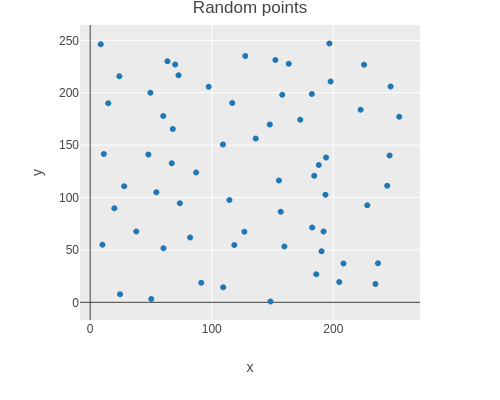
\includegraphics[width=.6\textwidth]{random-points}
  \end{center}
\end{frame}

\begin{frame}[fragile]
  \frametitle{Vector Modulus: Tests}
  \begin{minted}[]{clj}
(facts "Wrap around components of vector to be within -size/2..size/2"
       (mod-vec {:size 8} (vec2 2 3)) => (vec2 2 3)
       (mod-vec {:size 8} (vec2 5 2)) => (vec2 -3 2)
       (mod-vec {:size 8} (vec2 2 5)) => (vec2 2 -3)
       (mod-vec {:size 8} (vec2 -5 2)) => (vec2 3 2)
       (mod-vec {:size 8} (vec2 2 -5)) => (vec2 2 3)
       (mod-vec {:size 8} (vec3 2 3 1)) => (vec3 2 3 1)
       (mod-vec {:size 8} (vec3 5 2 1)) => (vec3 -3 2 1)
       (mod-vec {:size 8} (vec3 2 5 1)) => (vec3 2 -3 1)
       (mod-vec {:size 8} (vec3 2 3 5)) => (vec3 2 3 -3)
       (mod-vec {:size 8} (vec3 -5 2 1)) => (vec3 3 2 1)
       (mod-vec {:size 8} (vec3 2 -5 1)) => (vec3 2 3 1)
       (mod-vec {:size 8} (vec3 2 3 -5)) => (vec3 2 3 3))
  \end{minted}
\end{frame}

\begin{frame}[fragile]
  \frametitle{Vector Modulus: Implementation}
  \begin{minted}[]{clj}
(defn mod-vec
  [{:keys [size]} v]
  (let [size2 (/ size 2)
        wrap  (fn [x] (-> x (+ size2) (mod size) (- size2)))]
    (apply vec-n (map wrap v))))
  \end{minted}
\end{frame}

\begin{frame}[fragile]
  \frametitle{Modular Distance: Tests}
  \begin{minted}[]{clj}
(tabular "Wrapped distance of two points"
         (fact (mod-dist {:size 8} (vec2 ?ax ?ay) (vec2 ?bx ?by))
               => ?result)
         ?ax ?ay ?bx ?by ?result
         0   0   0   0   0.0
         0   0   2   0   2.0
         0   0   5   0   3.0
         0   0   0   2   2.0
         0   0   0   5   3.0
         2   0   0   0   2.0
         5   0   0   0   3.0
         0   2   0   0   2.0
         0   5   0   0   3.0)
  \end{minted}
\end{frame}

\begin{frame}[fragile]
  \frametitle{Modular Distance: Implementation}
  \begin{minted}[]{clj}
(defn mod-dist
  [params a b]
  (mag (mod-vec params (sub b a))))
  \end{minted}
\end{frame}

\begin{frame}[fragile]
  \frametitle{Lookup with Wrap Around: Tests}
  \begin{minted}[]{clj}
(facts "Wrapped lookup of tensor values"
       (let [t (tensor/compute-tensor [4 6] vec2)]
         (wrap-get t 2 3) => (vec2 2 3)
         (wrap-get t 2 7) => (vec2 2 1)
         (wrap-get t 5 3) => (vec2 1 3)
         (wrap-get (wrap-get t 5) 3) => (vec2 1 3)))
  \end{minted}
\end{frame}

\begin{frame}[fragile]
  \frametitle{Lookup with Wrap Around: Implementation}
  \begin{minted}[]{clj}
(defn wrap-get
  [t & args]
  (let [indices (map mod args (dtype/shape t))]
    (if (> (count indices) (count args))
      (apply tensor/select t indices)
      (apply t indices))))
  \end{minted}
\end{frame}

\begin{frame}[fragile]
  \frametitle{Division Index}
  \begin{minted}[]{clj}
(facts "Convert coordinate to division index"
       (division-index {:cellsize 4} 3.5)  => 0
       (division-index {:cellsize 4} 7.5)  => 1
       (division-index {:cellsize 4} -0.5) => -1)

(defn division-index
  [{:keys [cellsize]} x]
  (int (floor (/ x cellsize))))
  \end{minted}
\end{frame}

\begin{frame}
  \frametitle{Neighbouring Indices}
  \begin{center}
    \movie[width=13cm,height=7.6cm,showcontrols]{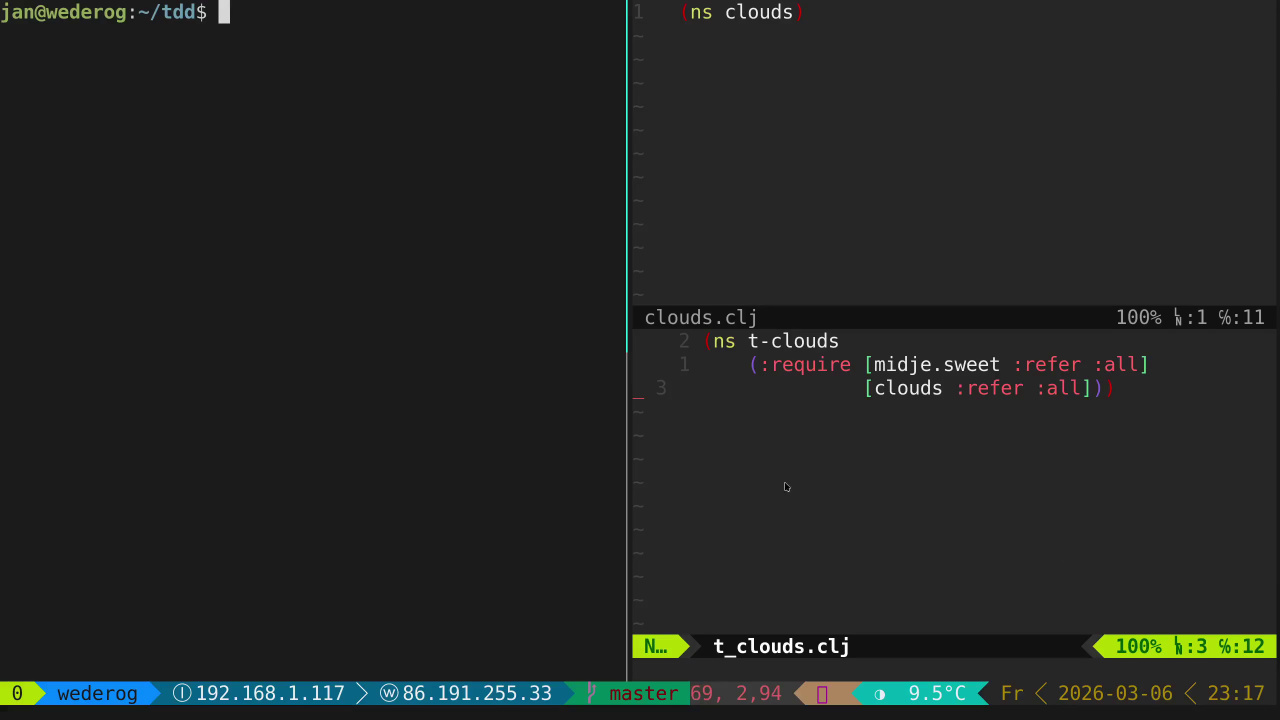
\includegraphics[width=13cm]{clojure-clouds-tdd}}{clojure-clouds-tdd.avi}
  \end{center}
\end{frame}

\begin{frame}[fragile]
  \frametitle{Worley Noise}
  \begin{minted}[]{clj}
(defn worley-noise
  [{:keys [size dimensions] :as params}]
  (let [random-points (random-points params)]
    (tensor/clone
      (tensor/compute-tensor
        (repeat dimensions size)
        (fn [& coords]
            (let [center   (map #(+ % 0.5) coords)
                  division (map (partial division-index params) center)]
              (apply min
                     (for [neighbour (apply neighbours division)]
                          (mod-dist params (apply vec-n (reverse center))
                                    (apply wrap-get
                                           random-points
                                           neighbour))))))
        :double))))
  \end{minted}
\end{frame}

\begin{frame}[fragile]
  \frametitle{Normalised Worley Noise}
  \begin{minted}[]{clj}
(def worley (worley-noise (make-noise-params 256 8 2)))

(def worley-norm
  (dfn/* (/ 255 (- (dfn/reduce-max worley) (dfn/reduce-min worley)))
         (dfn/- (dfn/reduce-max worley) worley)))

worley-norm
; #tech.v3.tensor<float64>[256 256]
; [[212,6 219,5 226,1 ... 191,0 198,3 205,5]
;  [214,6 221,9 229,2 ... 192,4 199,8 207,2]
;  [215,3 222,8 230,3 ... 192,8 200,3 207,8]
;  ...
;  [200,5 205,7 210,2 ... 182,4 188,7 194,8]
;  [205,3 211,0 216,2 ... 186,0 192,7 199,1]
;  [209,4 215,7 221,6 ... 188,9 195,9 202,7]]
  \end{minted}
\end{frame}

\begin{frame}
  \frametitle{Worley Noise Result}
  \begin{center}
    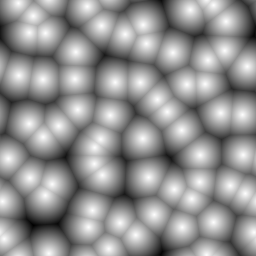
\includegraphics[width=.5\textwidth]{worley-noise}
  \end{center}
\end{frame}

\begin{frame}
  \frametitle{Perlin Noise}
  \begin{center}
    Perlin noise / Gradient noise
    \begin{itemize}
      \item Divide space into cell
      \item Assign a random gradient vector to each cell corner
      \item Compute dot product of distance vector and gradient vector
      \item Interpolate the dot product values to generate Perlin noise
    \end{itemize}
  \end{center}
\end{frame}

\begin{frame}[fragile]
  \frametitle{Random Gradient: Tests}
  \begin{minted}[]{clj}
(defn roughly-vec
  [expected error]
  (fn [actual]
      (<= (mag (sub actual expected)) error)))

(facts "Create unit vector with random direction"
   (with-redefs [rand (constantly 0.5)]
     (random-gradient 0 0)
     => (roughly-vec (vec2 (- (sqrt 0.5)) (- (sqrt 0.5))) 1e-6))
   (with-redefs [rand (constantly 1.5)]
     (random-gradient 0 0)
     => (roughly-vec (vec2 (sqrt 0.5) (sqrt 0.5)) 1e-6)))
  \end{minted}
\end{frame}

\begin{frame}[fragile]
  \frametitle{Random Gradient: Implementation}
  \begin{minted}[]{clj}
(defn random-gradient
[& args]
(loop [args args]
      (let [random-vector (apply vec-n
                                 (map (fn [_x] (- (rand 2.0) 1.0))
                                      args))
            vector-length (mag random-vector)]
        (if (and (> vector-length 0.0) (<= vector-length 1.0))
          (div random-vector vector-length)
          (recur args)))))
  \end{minted}
\end{frame}

\begin{frame}
  \frametitle{Perlin Noise Result}
  \begin{center}
    
\includegraphics[width=.5\textwidth]{perlin-noise}
  \end{center}
\end{frame}

\begin{frame}[fragile]
  \frametitle{Mixing Worley and Perlin Noise}
  \begin{minted}[]{clj}
(def perlin-worley-norm
  (dfn/+ (dfn/* 0.3 perlin-norm) (dfn/* 0.7 worley-norm)))
  \end{minted}
\end{frame}

\begin{frame}
  \frametitle{Mixing Worley and Perlin Noise}
  \begin{center}
    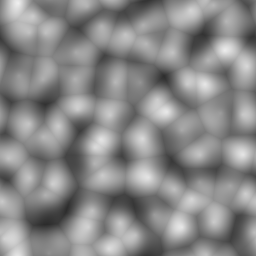
\includegraphics[width=.5\textwidth]{mixed-noise}
  \end{center}
\end{frame}

\begin{frame}
  \frametitle{OpenGL Superbible}
  \begin{center}
    
\includegraphics[width=.8\textwidth]{superbible}
  \end{center}
\end{frame}

\begin{frame}[fragile]
  \frametitle{Initialise OpenGL}
  \begin{minted}[]{clj}
(GLFW/glfwInit)
(def window-width 640)
(def window-height 480)
(GLFW/glfwDefaultWindowHints)
(GLFW/glfwWindowHint GLFW/GLFW_VISIBLE GLFW/GLFW_FALSE)
(def window (GLFW/glfwCreateWindow window-width window-height
                                   "Invisible Window" 0 0))
(GLFW/glfwMakeContextCurrent window)
(GL/createCapabilities)
  \end{minted}
\end{frame}

\begin{frame}[fragile]
  \frametitle{Offscreen Rendering}
  \begin{minted}[]{clj}
(defmacro render-array
  [width height & body]
  `(let [texture# (make-texture-2d ~width ~height)]
     (try
       (framebuffer-render texture# ~width ~height ~@body)
       (read-texture-2d texture# ~width ~height)
       (finally
         (GL11/glDeleteTextures texture#)))))
  \end{minted}
  \bigskip
  \begin{footnotesize}
    Complete source code at\ \url{https://clojurecivitas.org/volumetric_clouds/main.html}
  \end{footnotesize}
\end{frame}

\begin{frame}[fragile]
  \frametitle{Vertex and Fragment Shader}
  \begin{minted}[]{clj}
(def vertex-passthrough
"#version 130
in vec3 point;
void main()
{
  gl_Position = vec4(point, 1);
}")

(def fragment-test
"#version 130
out vec4 fragColor;
void main()
{
  // Render white pixels
  fragColor = vec4(1, 1, 1, 1);
}")
  \end{minted}
\end{frame}

\begin{frame}[fragile]
  \frametitle{Single Quad Vertex Array Object (VAO)}
  \begin{minted}[]{clj}
(defn setup-quad-vao
  []
  (let [vertices (float-array [ 1.0  1.0 0.0,
                               -1.0  1.0 0.0,
                                1.0 -1.0 0.0,
                               -1.0 -1.0 0.0])
        indices  (int-array [0 1 3 2])]
    (setup-vao vertices indices)))
  \end{minted}
\end{frame}

\begin{frame}[fragile]
  \frametitle{Vertex Attribute Memory Layout}
  \begin{minted}[]{clj}
(defn setup-point-attribute
  [program]
  (let [point-attribute (GL20/glGetAttribLocation program "point")]
    (GL20/glVertexAttribPointer point-attribute 3 GL11/GL_FLOAT false
                                (* 3 Float/BYTES) (* 0 Float/BYTES))
    (GL20/glEnableVertexAttribArray point-attribute)))
  \end{minted}
\end{frame}

\begin{frame}[fragile]
  \frametitle{Render a Test Pixel}
  \begin{minted}[]{clj}
(defn render-pixel
  [vertex-sources fragment-sources]
  (let [program (make-program-with-shaders vertex-sources fragment-sources)
        vao     (setup-quad-vao)]
    (setup-point-attribute program)
    (try
      (render-array 1 1
                    (GL20/glUseProgram program)
                    (GL11/glDrawElements GL11/GL_QUADS 4
                                         GL11/GL_UNSIGNED_INT 0))
      (finally
        (teardown-vao vao)
        (GL20/glDeleteProgram program)))))
  \end{minted}
\end{frame}

\begin{frame}[fragile]
  \frametitle{Render a White Pixel}
  \begin{minted}[]{clj}
(render-pixel [vertex-passthrough] [fragment-test])
; [1.0, 1.0, 1.0, 1.0]
  \end{minted}
\end{frame}

\begin{frame}[fragile]
  \frametitle{Noise Mock}
  \begin{minted}[]{clj}
(def noise-mock
"#version 130
float noise(vec3 idx)
{
  ivec3 v = ivec3(floor(idx.x), floor(idx.y), floor(idx.z)) % 2;
  return ((v.x == 1) == (v.y == 1)) == (v.z == 1) ? 1.0 : 0.0;
}")
  \end{minted}
\end{frame}

\begin{frame}[fragile]
  \frametitle{Noise Mock Probing Shader}
  \begin{minted}[]{clj}
(def noise-probe
  (template/fn [x y z]
"#version 130
out vec4 fragColor;
float noise(vec3 idx);
void main()
{
  fragColor = vec4(noise(vec3(<%= x %>, <%= y %>, <%= z %>)));
}"))
  \end{minted}
  \bigskip
  Using \href{https://github.com/weavejester/comb}{Comb} templating library
\end{frame}

\begin{frame}[fragile]
  \frametitle{Noise Mock Unit Tests}
  \begin{minted}[]{clj}
(tabular "Test noise mock"
         (fact (nth (render-pixel [vertex-passthrough]
                                  [noise-mock (noise-probe ?x ?y ?z)]) 0)
               => ?result)
         ?x ?y ?z ?result
         0  0  0  0.0
         1  0  0  1.0
         0  1  0  1.0
         1  1  0  0.0
         0  0  1  1.0
         1  0  1  0.0
         0  1  1  0.0
         1  1  1  1.0)
  \end{minted}
\end{frame}

\begin{frame}[fragile]
  \frametitle{Octave Weights}
  \begin{minted}[]{clj}
(defn octaves
  [n decay]
  (let [series (take n (iterate #(* % decay) 1.0))
        sum    (apply + series)]
    (mapv #(/ % sum) series)))

(octaves 4 0.5)
; [0.5333.. 0.2666.. 0.1333.. 0.0666..]
  \end{minted}
\end{frame}

\begin{frame}[fragile]
  \frametitle{Octaves of Noise: Probing Shader}
  \begin{minted}[]{clj}
(def octaves-probe
  (template/fn [x y z]
"#version 130
out vec4 fragColor;
float octaves(vec3 idx);
void main()
{
  fragColor = vec4(octaves(vec3(<%= x %>, <%= y %>, <%= z %>)));
}"))
  \end{minted}
\end{frame}

\begin{frame}[fragile]
  \frametitle{Octaves of Noise: Tests}
  \begin{minted}[]{clj}
(tabular "Test octaves of noise"
         (fact (first (render-pixel [vertex-passthrough]
                                    [noise-mock (noise-octaves ?octaves)
                                     (octaves-probe ?x ?y ?z)]))
               => ?result)
         ?x  ?y ?z ?octaves  ?result
         0   0  0  [1.0]     0.0
         1   0  0  [1.0]     1.0
         1   0  0  [0.5]     0.5
         0.5 0  0  [1.0]     0.0
         0.5 0  0  [0.0 1.0] 1.0
         1   0  0  [1.0 0.0] 1.0)
  \end{minted}
\end{frame}

\begin{frame}[fragile]
  \frametitle{Octaves of Noise: Implementation}
  \begin{minted}[]{clj}
(def noise-octaves
  (template/fn [octaves]
"#version 130
out vec4 fragColor;
float noise(vec3 idx);
float octaves(vec3 idx)
{
  float result = 0.0;
<% (doseq [multiplier octaves] %>
  result += <%= multiplier %> * noise(idx);
  idx *= 2.0;
<%= ) %>
  return result;
}"))
  \end{minted}
\end{frame}

\begin{frame}[fragile]
  \frametitle{Ray-Box-Intersection: Probing Shader}
  \begin{minted}[]{clj}
(def ray-box-probe
  (template/fn [ox oy oz dx dy dz]
"#version 130
out vec4 fragColor;
vec2 ray_box(vec3 box_min, vec3 box_max, vec3 origin, vec3 direction);
void main()
{
  vec3 box_min = vec3(-1, -1, -1);
  vec3 box_max = vec3(1, 1, 1);
  vec3 origin = vec3(<%= ox %>, <%= oy %>, <%= oz %>);
  vec3 direction = vec3(<%= dx %>, <%= dy %>, <%= dz %>);
  fragColor = vec4(ray_box(box_min, box_max, origin, direction), 0, 0);
}"))
  \end{minted}
\end{frame}

\begin{frame}[fragile]
  \frametitle{Ray-Box-Intersection: Tests}
  \begin{minted}[]{clj}
(tabular "Test intersection of ray with box"
   (fact ((juxt first second)
          (render-pixel [vertex-passthrough]
                        [ray-box (ray-box-probe ?ox ?oy ?oz ?dx ?dy ?dz)]))
         => ?result)
   ?ox ?oy ?oz ?dx ?dy ?dz ?result
   -2   0   0   1   0   0  [1.0 3.0]
   -2   0   0   2   0   0  [0.5 1.5]
   -2   2   2   1   0   0  [0.0 0.0]
    0  -2   0   0   1   0  [1.0 3.0]
    0  -2   0   0   2   0  [0.5 1.5]
    2  -2   2   0   1   0  [0.0 0.0]
    0   0  -2   0   0   1  [1.0 3.0]
    0   0  -2   0   0   2  [0.5 1.5]
    2   2  -2   0   0   1  [0.0 0.0]
    0   0   0   1   0   0  [0.0 1.0]
    2   0   0   1   0   0  [0.0 0.0])
  \end{minted}
\end{frame}

\begin{frame}[fragile]
  \frametitle{Ray-Box-Intersection: Implementation}
  \begin{minted}[]{clj}
(def ray-box
"#version 130
vec2 ray_box(vec3 box_min, vec3 box_max, vec3 origin, vec3 direction)
{
  vec3 inv_dir = 1.0 / direction;
  vec3 smin = (box_min - origin) * inv_dir;
  vec3 smax = (box_max - origin) * inv_dir;
  vec3 s1 = min(smin, smax);
  vec3 s2 = max(smin, smax);
  float s_near = max(max(s1.x, s1.y), s1.z);
  float s_far = min(min(s2.x, s2.y), s2.z);
  if (isinf(s_near) || isinf(s_far))
    return vec2(0.0, 0.0);
  else
    return vec2(max(s_near, 0.0), max(0.0, s_far));
}")
  \end{minted}
\end{frame}

\begin{frame}[fragile]
  \frametitle{Placeholder Shaders}
  \begin{center}
    \begin{minipage}{0.48\textwidth}
      \begin{minted}[]{clj}
(def fog
  (template/fn [v]
"#version 130
float fog(vec3 idx)
{
  return <%= v %>;
}"))
      \end{minted}
    \end{minipage}
    \begin{minipage}{0.48\textwidth}
      \begin{minted}[]{clj}
(def no-shadow
"#version 130
float shadow(vec3 point)
{
  return 1.0;
}")
      \end{minted}
    \end{minipage}\bigskip\\
    \begin{minipage}{0.48\textwidth}
      \begin{minted}[]{clj}
(def constant-scatter
"#version 130
float in_scatter(vec3 point, vec3 direction)
{
  return 1.0;
}")
      \end{minted}
    \end{minipage}
  \end{center}
\end{frame}

\begin{frame}[fragile]
  \frametitle{Cloud Transfer Probe}
  \begin{minted}[]{clj}
(def cloud-transfer-probe
  (template/fn [a b]
"#version 130
out vec4 fragColor;
vec4 cloud_transfer(vec3 origin, vec3 direction, vec2 interval);
void main()
{
  vec3 origin = vec3(0, 0, 0);
  vec3 direction = vec3(1, 0, 0);
  vec2 interval = vec2(<%= a %>, <%= b %>);
  fragColor = cloud_transfer(origin, direction, interval);
}"))
  \end{minted}
\end{frame}

\begin{frame}[fragile]
  \frametitle{Cloud Transfer Tests}
  \begin{minted}[]{clj}
(tabular "Test cloud transfer"
         (fact (seq (render-pixel [vertex-passthrough]
                                  [(fog ?density) constant-scatter no-shadow
                                   (cloud-transfer "fog" ?step)
                                   (cloud-transfer-probe ?a ?b)]))
               => (roughly-vector ?result 1e-3))
         ?a ?b ?step ?density ?result
         0  0  1     0.0      [0.0 0.0 0.0 0.0]
         0  1  1     1.0      [0.632 0.632 0.632 0.632]
         0  1  0.5   1.0      [0.632 0.632 0.632 0.632]
         0  1  0.5   0.5      [0.393 0.393 0.393 0.393])
  \end{minted}
\end{frame}

\begin{frame}[fragile]
  \frametitle{Cloud Transfer Shader}
  \begin{footnotesize}
    \begin{minted}[]{clj}
(def cloud-transfer
  (template/fn [noise step]
"#version 130
#define STEP <%= step %>
float <%= noise %>(vec3 idx);
float in_scatter(vec3 point, vec3 direction);
float shadow(vec3 point);
vec4 cloud_transfer(vec3 origin, vec3 direction, vec2 interval)
{
  vec4 result = vec4(0, 0, 0, 0);
  for (float t = interval.x + 0.5 * STEP; t < interval.y; t += STEP) {
    vec3 point = origin + direction * t;
    float density = <%= noise %>(point);
    float transmittance = exp(-density * STEP);
    vec3 color = vec3(in_scatter(point, direction) * shadow(point));
    result.rgb += color * (1.0 - result.a) * (1.0 - transmittance);
    result.a = 1.0 - (1.0 - result.a) * transmittance;
  };
  return result;
}"))
    \end{minted}
  \end{footnotesize}
\end{frame}

\begin{frame}[fragile]
  \frametitle{Scene Fragment Shader}
  \begin{footnotesize}
    \begin{minted}[]{clj}
(def fragment-cloud
"#version 130
uniform vec2 resolution;
uniform vec3 light;
uniform mat3 rotation;
uniform float focal_length;
uniform float distance;
out vec4 fragColor;
vec2 ray_box(vec3 box_min, vec3 box_max, vec3 origin, vec3 direction);
vec4 cloud_transfer(vec3 origin, vec3 direction, vec2 interval);
void main()
{
  vec3 direction =
    normalize(rotation * vec3(gl_FragCoord.xy - 0.5 * resolution, focal_length));
  vec3 origin = rotation * vec3(0, 0, -distance);
  vec2 interval = ray_box(vec3(-0.5, -0.5, -0.5), vec3(0.5, 0.5, 0.5), origin, direction);
  vec4 transfer = cloud_transfer(origin, direction, interval);
  vec3 background = mix(vec3(0.125, 0.125, 0.25), vec3(1, 1, 1),
                        pow(dot(direction, light), 1000.0));
  fragColor = vec4(background * (1.0 - transfer.a) + transfer.rgb, 1.0);
}")
    \end{minted}
  \end{footnotesize}
\end{frame}

\begin{frame}[fragile]
  \frametitle{Scene Render Method}
  \begin{minted}[]{clj}
(defn render-fog
  [width height]
  (let [fragment-sources [ray-box constant-scatter no-shadow
                          (cloud-transfer "fog" 0.01) (fog 1.0)
                          fragment-cloud]
        program          (make-program-with-shaders [vertex-passthrough]
                                                    fragment-sources)
        vao              (setup-quad-vao)]
    (setup-point-attribute program)
    (try
      (render-array width height
                    (setup-fog-uniforms program width height)
                    (GL11/glDrawElements GL11/GL_QUADS 4
                                         GL11/GL_UNSIGNED_INT 0))
      (finally
        (teardown-vao vao)
        (GL20/glDeleteProgram program)))))
  \end{minted}
\end{frame}

\begin{frame}
  \frametitle{Constant Fog}
  \begin{center}
    
\includegraphics[width=.65\textwidth]{fog}
  \end{center}
\end{frame}

\begin{frame}[fragile]
  \frametitle{3D Noise Texture}
  \begin{minted}[]{clj}
(def noise3d (dfn/- (dfn/* 0.3 (perlin-noise (make-noise-params 32 4 3)))
                    (dfn/* 0.7 (worley-noise (make-noise-params 32 4 3)))))

(def noise-3d-norm (dfn/* (/ 1.0 (- (dfn/reduce-max noise3d)
                                    (dfn/reduce-min noise3d)))
                          (dfn/- noise3d (dfn/reduce-min noise3d))))

(def noise-texture
  (float-array->texture3d (dtype/->float-array noise-3d-norm) 32))
  \end{minted}
\end{frame}

\begin{frame}[fragile]
  \frametitle{Noise Shader}
  \begin{minted}[]{clj}
(def noise-shader
"#version 130
uniform sampler3D noise3d;
float noise(vec3 idx)
{
  return texture(noise3d, idx).r;
}")
  \end{minted}
\end{frame}

\begin{frame}[fragile]
  \frametitle{Generic Scene Render Method}
  \begin{minted}[]{clj}
(defn render-noise
  [width height & cloud-shaders]
  (let [fragment-sources (concat cloud-shaders [ray-box fragment-cloud])
        program          (make-program-with-shaders [vertex-passthrough] 
                                                    fragment-sources)
        vao              (setup-quad-vao)]
    (try
      (setup-point-attribute program)
      (render-array width height
                    (setup-noise-uniforms program width height)
                    (GL11/glDrawElements GL11/GL_QUADS 4
                                         GL11/GL_UNSIGNED_INT 0))
      (finally
        (teardown-vao vao)
        (GL20/glDeleteProgram program)))))
  \end{minted}
\end{frame}

\begin{frame}[fragile]
  \frametitle{3D Noise}
  \begin{minted}[]{clj}
(rgba-array->bufimg
  (render-noise 640 480
                constant-scatter no-shadow (cloud-transfer "noise" 0.01)
                noise-shader)
  640 480)
  \end{minted}
\end{frame}

\begin{frame}
  \frametitle{3D Noise}
  \begin{center}
    
\includegraphics[width=.65\textwidth]{noise}
  \end{center}
\end{frame}

\begin{frame}[fragile]
  \frametitle{Remapped Noise}
  \begin{minted}[]{clj}
(rgba-array->bufimg
  (render-noise 640 480
                constant-scatter no-shadow
                (cloud-transfer "remap_noise" 0.01)
                remap-clamp (remap-noise "noise" 0.45 0.9 cloud-strength)
                noise-shader)
  640 480)
  \end{minted}
\end{frame}

\begin{frame}
  \frametitle{Remapped Noise}
  \begin{center}
    
\includegraphics[width=.65\textwidth]{remap}
  \end{center}
\end{frame}

\begin{frame}[fragile]
  \frametitle{Octaves of Noise}
  \begin{minted}[]{clj}
(rgba-array->bufimg
  (render-noise 640 480 constant-scatter no-shadow
                (cloud-transfer "remap_noise" 0.01)
                remap-clamp (remap-noise "octaves" 0.45 0.9 cloud-strength)
                (noise-octaves (octaves 4 0.5)) noise-shader)
  640 480)
  \end{minted}
\end{frame}

\begin{frame}
  \frametitle{Octaves of Noise}
  \begin{center}
    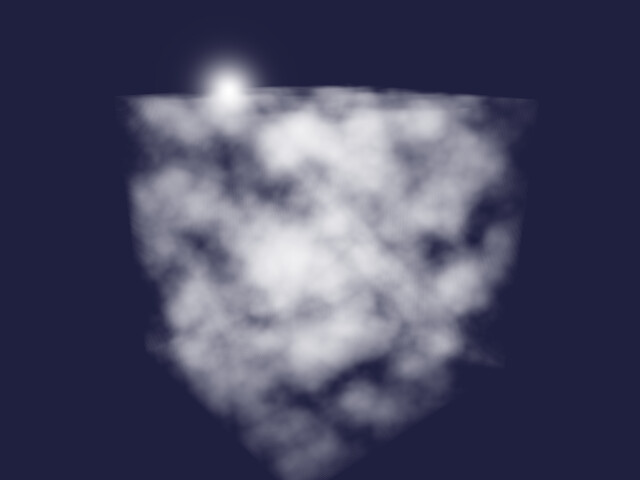
\includegraphics[width=.65\textwidth]{octaves}
  \end{center}
\end{frame}

\begin{frame}[fragile]
  \frametitle{Mie Scattering}
  \begin{minted}[]{clj}
(def mie-scatter
  (template/fn [g]
"#version 450 core
#define M_PI 3.1415926535897932384626433832795
#define ANISOTROPIC 0.25
#define G <%= g %>
uniform vec3 light;
float mie(float mu)
{
  return 3 * (1 - G * G) * (1 + mu * mu) /
    (8 * M_PI * (2 + G * G) * pow(1 + G * G - 2 * G * mu, 1.5));
}
float in_scatter(vec3 point, vec3 direction)
{
  return mix(1.0, mie(dot(light, direction)), ANISOTROPIC);
}"))
  \end{minted}
\end{frame}

\begin{frame}[fragile]
  \frametitle{Mie Probe}
  \begin{minted}[]{clj}
(def mie-probe
  (template/fn [mu]
"#version 450 core
out vec4 fragColor;
float mie(float mu);
void main()
{
  float result = mie(<%= mu %>);
  fragColor = vec4(result, 0, 0, 1);
}"))

(defn scatter-amount [theta]
  (first (render-pixel [vertex-passthrough]
                       [(mie-scatter 0.76) (mie-probe (cos theta))])))
  \end{minted}
\end{frame}

\begin{frame}
  \frametitle{Mie Scattering}
  \begin{center}
    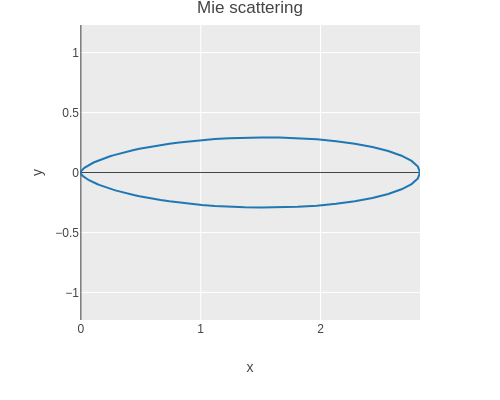
\includegraphics[width=.6\textwidth]{mie-scatter}
  \end{center}
\end{frame}

\begin{frame}[fragile]
  \frametitle{Mie Scattering}
  \begin{minted}[]{clj}
(rgba-array->bufimg
  (render-noise 640 480 (mie-scatter 0.76) no-shadow
                (cloud-transfer "remap_noise" 0.01)
                remap-clamp (remap-noise "octaves" 0.45 0.9 cloud-strength)
                (noise-octaves (octaves 4 0.5)) noise-shader)
  640 480)
  \end{minted}
\end{frame}

\begin{frame}
  \frametitle{Mie Scattering}
  \begin{center}
    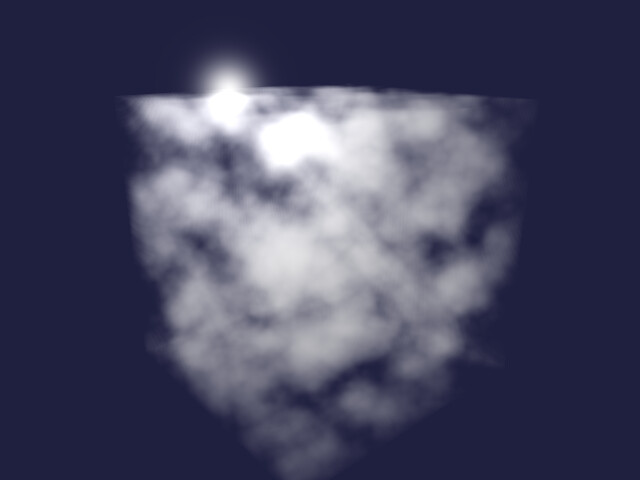
\includegraphics[width=.65\textwidth]{scattering}
  \end{center}
\end{frame}

\begin{frame}[fragile]
  \frametitle{Shadow Shader}
  \begin{minted}[]{clj}
(def shadow
  (template/fn [noise step]
"#version 130
#define STEP <%= step %>
uniform vec3 light;
float <%= noise %>(vec3 idx);
vec2 ray_box(vec3 box_min, vec3 box_max, vec3 origin, vec3 direction);
float shadow(vec3 point)
{
  vec2 interval = ray_box(vec3(-0.5, -0.5, -0.5), vec3(0.5, 0.5, 0.5),
                          point, light);
  float result = 1.0;
  for (float t = interval.x + 0.5 * STEP; t < interval.y; t += STEP) {
    float density = <%= noise %>(point + t * light);
    float transmittance = exp(-density * STEP);
    result *= transmittance;
  };
  return result;
}"))
  \end{minted}
\end{frame}

\begin{frame}
  \frametitle{Shadows}
  \begin{center}
    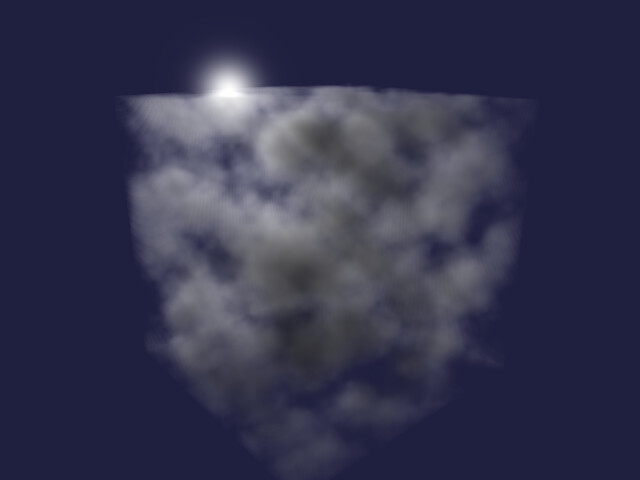
\includegraphics[width=.65\textwidth]{shadows}
  \end{center}
\end{frame}

\end{document}
